%------------------------------------------------------------------------------
\documentclass[a4paper,10pt]{article}
%------------------------------------------------------------------------------

\usepackage{amssymb}
\usepackage{amsmath}
\usepackage{graphicx}

% Some math operators
\DeclareMathOperator{\Div}{div}
\DeclareMathOperator{\Grad}{grad}
\newcommand{\inner}[2]{\langle #1, #2 \rangle}
\newcommand{\R}{\mathbb{R}}
\newcommand{\foralls}{\forall\,}
\newcommand{\ddt}[1]{{#1}_t}
\newcommand{\dx}{\dif{}x}
\newcommand{\ds}{\dif{}s}
\newcommand{\dS}{\dif{}S}
\newcommand{\tr}{\mbox{tr}}
\newcommand{\eps}{\epsilon}

\begin{document}
\section{Homogenous growth in a unit cube}
We want to test growth model proposed by Kerckhoffs et al (2012) in the simplest possible setting; a 
homogenous unit cube subjected to uni-axial stretch. With a suitable choice of boundary conditions, this case gives a 
uniform deformation state consequently uniform growth, and the equilibrium PDEs can be reduced to simple
algebraic relations. 

\subsection{Unit cube with no growth}
For simplicity, we first compute the relevant kinematic quantities for the case with no growth. 
We consider a unit cube with fibers aligned in the $x$-direction. One side of the cube, for $x=0$, is 
restricted from moving in the $x$-direction. The opposite side, $x=1$, is subjected to a uniform
displacement $u_0 > 0$. The remaining four sides of the cube are unloaded, i.e., homogenous 
Neumann conditions. We also apply (minimal) boundary conditions to eliminate rigid body motion, and assume
that the material is fully incompressible. 

These choices give rise to a uniform
deformation field with a diagonal deformation gradient with components
$F_{11} = \lambda = 1+u_0, F_{22}=F_{33} = \sqrt{1/\lambda}$.
The right Cauchy-Green tensor $C$ and the Green-Lagrange tensor
$E$ will also be diagonal, with components $C_{11} = \lambda^2 , 
C_{22} =C_{33} = 1/\lambda,  
E_{11} = \frac{1}{2}(\lambda^2 - 1)$, and 
$E_{22} = E_{33} = \frac{1}{2}(\frac{1}{\lambda}-1).$

The growth model by Kerckhoffs et al relies on the maximum fiber strain and the maximum principal strain 
in the transverse plane. With the simple deformation state given above, the fiber strain is given by
\[
  E_{ff} = E_{11} = \frac{1}{2}(\lambda^2 - 1),
\]
and since the strain tensor is diagonal, the maximum principal strain $E_{cross,max}$ is given 
\[
  E_{cross,max} = E_{22} = E_{33} =  \frac{1}{2}(\frac{1}{\lambda}-1).
\]

\subsection{Volumetric growth}
In the volumetric growth framework introduced by 
Rodriguez et al (1995), the total deformation $F$ is decomposed into an elastic component $F_e$ and a growth
component $F_g$, according to:
\[
  F = F_e F_g . 
\]
The growth deformation $F_g$ is assumed to be stress-free, and can be viewed as a transition from one stress-free 
equilibrium configuration to another. If the new equilibrium configuration is compatible (e.g., does not create
overlapping materials or gaps) and satisfies the applied boundary conditions, we will have $F_e = I$, $F=F_g$, and the
material has simply grown to a new stress-free configuration. An artificial example of such growth may be the unit cube 
defined above, with the side $x=1$ unloaded, and prescribed growth $\lambda_g$ in the $x$-direction. 
We then have $F=F_g= diag(\lambda_g, 1, 1)$, with $\lambda_g > 1$, and the
material simply gets longer in the $x$-direction with no associated stresses. If, however, the unit cube was completely 
constrained from deforming in all directions, we would have $F = I$, $F_g= diag(\lambda_g, 1, 1)$, and 
$F_e = F F_g^{-1} = diag(1/\lambda_g, 1, 1)$, which will typically result in a non-zero stress state. 

The growth law proposed by Kerckhoffs et al is formulated in terms of the growth stimuli $s_l$ and $s_t$, 
which stimulate longitudinal (fiber) and transversal growth, respectively. These are based on pre-defined
set points $E_{ff,set}, E_{cross,set}$ for the strains $E_{ff}, E_{cross,max}$ defined above:
\begin{align*}
  s_l &= \max(E_{ff}) - E_{ff,set}, \\
  s_t &= \min(E_{cross,max}) - E_{cross,set} .
\end{align*}
Here, it is important to note that the growth stimuli are computed from the \emph{elastic} component of the strain,
i.e., the quantities $E_{ff}, E_{cross,max}$ are computed from $F_e$ and not total deformation gradient $F$. 
Specifically, in the context of volumetric growth we have the relevant stretch and strain tensors defined by:
\begin{align*}
  C &= F_e^TF_e ,\\
  E &= 1/2(C - I) .
\end{align*}
The growth tensor $F_g$ is then defined in terms of incremental growth tensors $F_{g,i}$, which represent the
growth over a single growth step. The incremental growth tensor is given  
by $F_{g,i}= diag(F_{g,i,ff}, F_{g,i,cross}, F_{g,i,cross})$, with the components 
$F_{g,i,ff}, F_{g,i,cross}$ defined by eqs (8) and (9) in Kerckhoffs et al (2012). The cumulative growth tensor
after $n$ steps is then defined as $F_g^n = F_g^{n-1} F_{g,i}$.

\subsubsection{Initial tests}
Before running an actual growth test, it is useful to get an idea of what the various functions defining the
growth look like. Figure \ref{fig:k_functions} shows the functions $k_{ff}, k_{cc}$ (eqs (11) and (12) from Kerckhoffs et al)
as functions of the cumulative growth. The functions behave as expected, effectively stopping the growth as 
the overall growth limits are reached. Figure \ref{fig:incr_growth_tensors} shows the incremental growth tensor components
as functions of the growth stimuli. Here, we assume that the cumulative growth is below the limit, so $k_{ff} = k_{cc} = 1$.
The set points are chosen as $E_{ff, set} = E_{cross,set} = 0$, the time step $\Delta t_{growth} = 1$, 
and all other parameters are as given in Table 2 of Kerckhoffs et al.  
\begin{figure}
  \centerline{
    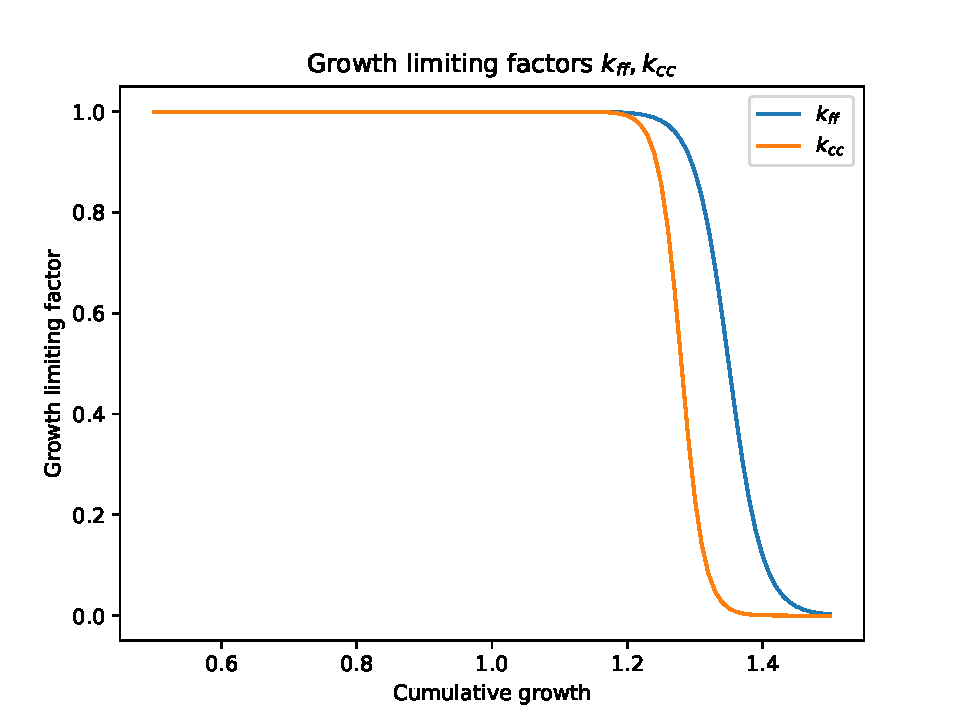
\includegraphics{figs/k_functions}
  }
\caption{The growth limiting factors $k_{ff}, k_{cc}$ as functions of cumulative growth.}
\label{fig:k_functions}
\end{figure}

\begin{figure}
  \centerline{
    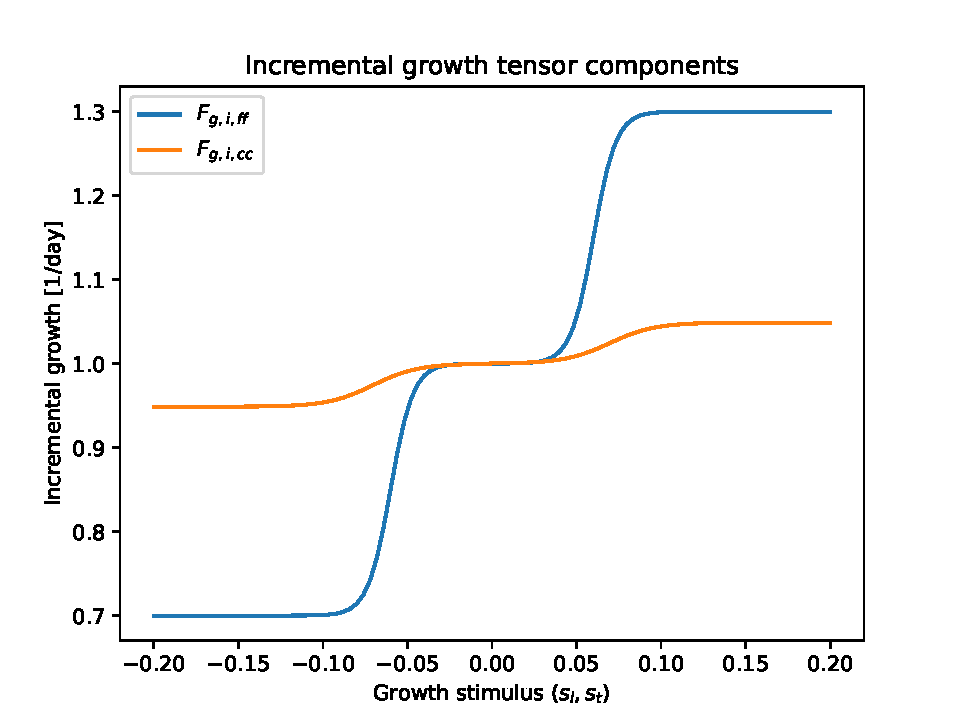
\includegraphics{figs/incr_growth_tensor}
  }
\caption{The incremental growth tensor components $F_{g,i,ff}, F_{g,i,cc}$, as functions of the growth stimuli $s_l, s_t$.} 
\label{fig:incr_growth_tensors}
\end{figure}

\subsubsection{Growth of the unit cube}
We now return to the unit cube subjected to uni-axial stretch $\lambda$, as defined above. With $\lambda > 1$, the cube 
should grow in the longitudinal direction and shrink in the transverse direction, and the growth should converge towards
an equilibrium where the elastic strain components $E_{ff}$ and $E_{cross,max}$ are equal to the set point values.
Figure \ref{fig:cum_growth_tensors} shows the fiber and transverse growth tensor components as functions of time, 
measured in days, for uniaxial constant stretch $\lambda = 1.1$, and set points $E_{ff, set} = E_{cross,set} = 0$. 
For this case the growth tensor $F_g$ should converge towards the overall tensor $F$, for which $F_e = I$ and 
$E_{ff} = E_{cross,max} = 0$.  In the limit we should have $F_g = F = diag(\lambda, \sqrt{1/\lambda}, sqrt{1/\lambda})$. 


Note: While both curves seem to converge towards the right values, the longitudinal growth curve is extremely steep at 
the start. This looks a bit strange, and it is worth double-checking the code and the parameters to confirm that this is correct.
However, judging from the parameters in the original paper it may be correct. The maximal growth ($f_{ff,max}$) is 0.3 (day$^{-1}$), 
and the value of the stimulus that gives 50\% of maximal growth ($s_{l,50}$) is 0.06. So, only 6\% longitudinal strain should give a 
longitudinal growth of about 0.15 per day. 

\begin{figure}
  \centerline{
    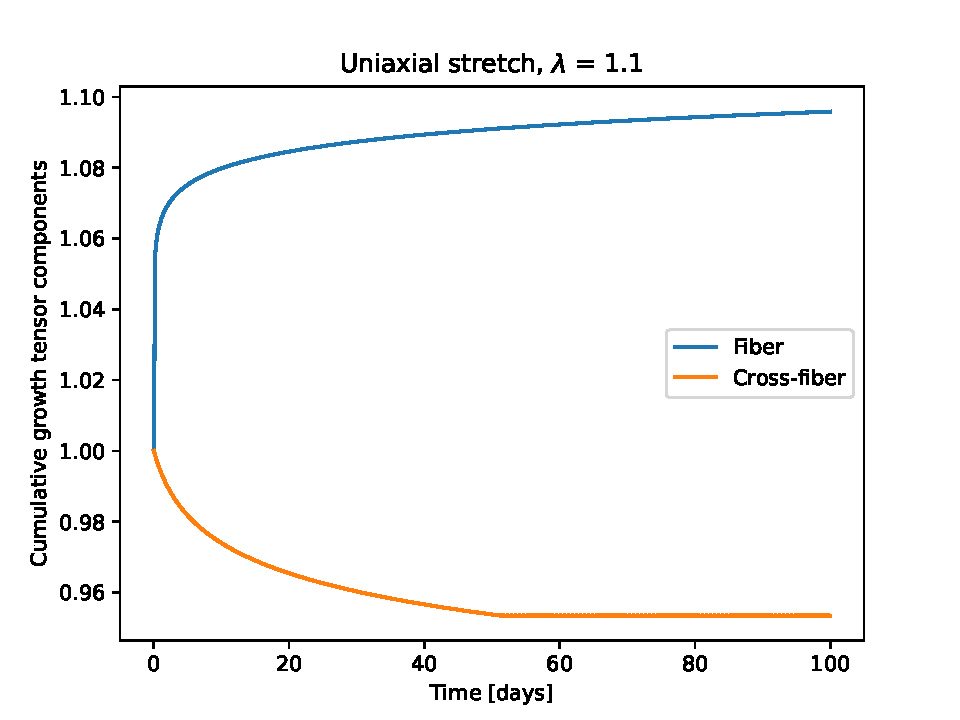
\includegraphics{figs/cumulative_growth}
  }
\caption{The cumulative growth tensor components $F_{g,i,ff}, F_{g,i,cc}$ as functions of time.}
\label{fig:cum_growth_tensors}
\end{figure}

\end{document}